\section{Research methodology}
This research is not of a thoroughly theoretical nature, its more of an exploratory/explanatory nature, see what happens under some conditions and explain the correlation.

The development process from Heath et al.~\cite{heath2009survey} (figure~\ref{fig:steps_simulation}) has been followed.

The process consists of several rounds.

\paragraph{Formulating the problem and objectives}
The first round consists of the formulation of the problem and setting the objectives.
This is already complete, they are mentioned as the research goals in the previous section.

\paragraph{Conceptional validation}
The second round consists of building and validating the conceptual model.
It relies upon known system theories, drives model development and dictates the variety of assumptions required in any model abstraction process.
The conceptual model forms the foundation of an ABM model; an invalid conceptual model indicates the model may not be an appropriate representation of reality~\cite{heath2009survey}.

The conceptional model consists of which agents exist and the description of their behaviour rules.
The model based approach is a way to eliminate all variables not direct related to the problem and keep only the essence of the situation.

All other interesting variables must be defined, such as simulation period, hourly wage, number of agents of each type.

The environment where multiple agents act is called a multi-agent system end the problem is called a multi-agent planning problem (from~\cite{russell2016artificial}).

\paragraph{Translate into computer model}
This round converts the conceptional model into computer code.
The environment used in this study is NetLogo.

A large part of the world is bases on an existing model,i.e., the Taxi Cab model~\cite{dongpingtaxicabs2019} as shown in figure~\ref{fig:taxi cab}
\begin{figure}
    \centering
    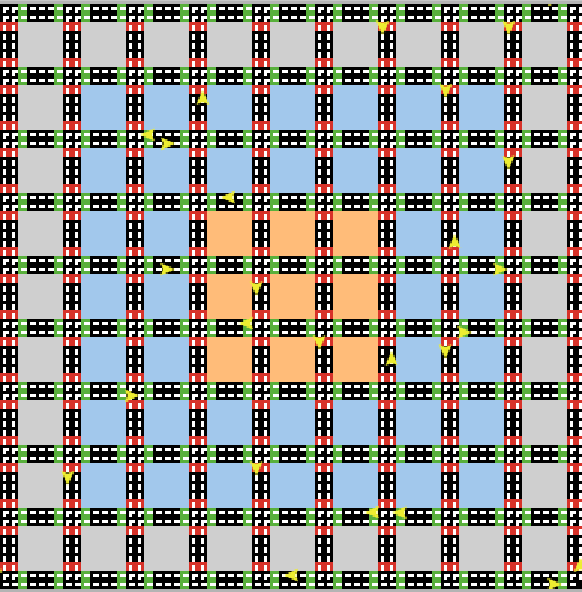
\includegraphics[width=6cm]{sections/pics/Taxi Cabs}
    \caption{Taxi Cab Model}
    \label{fig:taxi cab}
\end{figure}

This model has a street pattern on which agents can move, this will be reused in this study.
The agents behavior though is different and is new.


\paragraph{Run simulations and obtain results}
With the ready model, simulations will be run.
The results will be presented as graphs and tables.
The results will be analysed and be compared.







